% options:
% thesis=B bachelor's thesis
% thesis=M master's thesis
% czech thesis in Czech language
% slovak thesis in Slovak language
% english thesis in English language
% hidelinks remove colour boxes around hyperlinks

\documentclass[thesis=M,czech]{FITthesis}[2012/06/26]

\usepackage[utf8]{inputenc} % LaTeX source encoded as UTF-8

\usepackage{float}

\usepackage{graphicx} %graphics files inclusion
% \usepackage{amsmath} %advanced maths
% \usepackage{amssymb} %additional math symbols

\usepackage{dirtree} %directory tree visualisation

% % list of acronyms
% \usepackage[acronym,nonumberlist,toc,numberedsection=autolabel]{glossaries}
% \iflanguage{czech}{\renewcommand*{\acronymname}{Seznam pou{\v z}it{\' y}ch zkratek}}{}
% \makeglossaries

\newcommand{\tg}{\mathop{\mathrm{tg}}} %cesky tangens
\newcommand{\cotg}{\mathop{\mathrm{cotg}}} %cesky cotangens

% % % % % % % % % % % % % % % % % % % % % % % % % % % % % % 
% ODTUD DAL VSE ZMENTE
% % % % % % % % % % % % % % % % % % % % % % % % % % % % % % 

\department{Katedra softwarového inženýrství}
\title{Vývoj FIORI aplikace nad SAP PM modulem pro realizaci servisních zakázek a preventivní údržby}
\authorGN{Marcel} %(křestní) jméno (jména) autora
\authorFN{Morávek} %příjmení autora
\authorWithDegrees{Bc. Marcel Morávek} %jméno autora včetně současných akademických titulů
\author{Marcel Morávek} %jméno autora bez akademických titulů
\supervisor{Ing. Martin Šindlář}
\acknowledgements{Poděkování}
\abstractCS{Abstrakt CZ}
\abstractEN{Abstrakt EN}
\placeForDeclarationOfAuthenticity{V~Praze}
\declarationOfAuthenticityOption{4} %volba Prohlášení (číslo 1-6)
\keywordsCS{SAP, Fiori}
\keywordsEN{SAP, Fiori}
% \website{http://site.example/thesis} %volitelná URL práce, objeví se v tiráži - úplně odstraňte, nemáte-li URL práce

\setcounter{secnumdepth}{5}

\begin{document}

% \newacronym{CVUT}{{\v C}VUT}{{\v C}esk{\' e} vysok{\' e} u{\v c}en{\' i} technick{\' e} v Praze}
% \newacronym{FIT}{FIT}{Fakulta informa{\v c}n{\' i}ch technologi{\' i}}

\begin{introduction}
	Tato práce se zaobírá ...
\end{introduction}

\chapter{Cíl práce}
Cílem této práce je vytvoření webové SAP Fiori aplikace nad SAPovským modulem údržby ve frameworku SAPUI5. Pomocí této aplikace bude umožněno realizovat servisní zakázky i preventivní údržbu strojů a to včetně jejich vybavení.

\section{Vývojová část}
Cílem praktické části je navržení uživatelského rozhraní aplikace s ohledem na způsob zacházení s modulem údržby. Nadále pak implementace samotné aplikace dle provedeného návrhu. 

\section{Rešeršní část}
Jedním z cílů rešeršní části je porovnání prostředí podporujících vývoj ve frameworku SAPUI5. 

\section{Co není cílem práce}
Cílem této práce není implementace ani návrh funkčnosti uvnitř EPRového systému. Tato práce začíná na úrovni komunikačních rozhraní jednotlivých funkčních modulů realizujících požadované operace. 

\chapter{SAP}
Tata kapitola se věnuje podnikovému informačnímu systému SAP. V jednotlivých podkapitolách jsou pak popsány obecné informace o historii firmy a architektonické struktuře systému. Dále jsou zde popsány i jednotlivé technické komponenty, které jsou použity pro realizaci požadované aplikace. 
\section{Společnost SAP}
Společnost SAP je v současné době jedním z největších poskytovatelů podnikových aplikací a jednou z největších softwarových společností na celém světe. 
Pod zkratkou SAP se schovávají počáteční písmena německých slov „Systeme, Anwendungen, Produkte in der Datenverarbeitung“. Anglicky si lze zkratku přeložit pomocí anglických slov „Systems - Applications - Products in data processing“.

\section{SAP R3}

První verze systému, která přišla na svět v roce 1973, SAP R/1, byla tvořena finančním účetnictvím. Další verze SAP R/2 již můžeme nazývat za první funkční ERP systém (Enterprise resources planning), ovšem nevýhodou tohoto systému byla nutnost využívání sálových počítačů. Verzí SAP R/3 z roku 1992 byla změněna architektura SAPu, kdy se zaměnily sálové počítače na architekturu klient-server a začaly se využívat relační databáze. Výhoda této architektury byla především v kompatibilitě s různými platformami a operačními systémy Microsoft Windows nebo Unix. Další verze byla v roce 2002 spuštěna pod názvem SAP R/3 Enterprise. V roce 2004 byly nově uspořádány komponenty, čímž vznikl centrální produkt mySAP Business Suite. Došlo k oddělení aplikačních komponent od technických, přičemž se nadále označují jako SAP NetWeaver.

Příchodem verze SAP R/3 se změnila architektura SAPu na architekturu klient-server, která je tvořena třemi vrstvami:
\begin{itemize}
	\item
	\textbf{Prezenční vrstva} - Prezenční vrstva slouží pro komunikaci mezi uživatelem a počítačem. Vlastní komunikace probíhá na klientské části – prezentačním serveru. Nedílnou součástí prezentačního serveru je SAP GUI rozhraní, které se stará o komunikaci mezi prezentačním a aplikačním serverem.
	\item
	\textbf{Aplikační vrstva} - Aplikační vrstva je tvořena aplikačním serverem, který jednak přes SAP GUI komu-nikuje s klientem a jednak komunikuje s databází přes systém pro správu databáze. Vlastní programy, vytvořené v systému ABAP, jsou uloženy na aplikačních serverech.
	\item
	\textbf{Databázová vrstva} - Databázová vrstva je tvořena vlastními databázovými servery, které slouží pro ukládání dat. Jelikož SAP je multiplatformní systém, vývojáře nemusí zajímat, na jaké databázové platformě (UNIX, ORACLE, SUN, MICROSOFT) databázová vrstva běží, aplikační vrstva bude vypadat vždy stejně.
\end{itemize} 	

\subsection{Moduly SAP R3}
Systém SAP R/3 je vnitřně rozdělen do několika různých modulů. Každý z nich pak řeší konkrétní problematiku firmy.

\begin{itemize}
	\item
	\textbf{Financial Accounting (FI)} označuje finanční účetnictví a je jedním z nejdůležitějších modulů SAP ERP. Používá se k uložení finančních dat organizace a pomáhá analyzovat finanční podmínky společnosti na trhu.
	\item
	\textbf{Controlling (CO)} podporuje koordinaci, monitorování a optimalizaci všech procesů v organizaci. Zahrnuje správu a konfiguraci základních dat, které pokrývají náklady a výnosy, interní objednávky a další nákladové prvky a funkční oblasti. Jeho hlavním účelem je plánování. Umožňuje určit odchylky srovnáním skutečných dat s údaji plánu a tím umožňuje řídit obchodní toky v organizaci.
	\item
	\textbf{Asset Management (AM)} slouží k optimální správě fyzického majetku organizace. Zahrnuje takové funkcionality jako jsou návrh, konstrukce, provoz, údržba a výměna zařízení. Spravuje majetek v jednotlivých odděleních (obchodních jednotkách).
	\item
	\textbf{Project system (PS)} - Plánování dlouhodobých projektů
	\item
	\textbf{Workflow (WF)} - Řízení oběhu dokumentů
	\item
	\textbf{Industry Solutions (IS)} - Specifická řešení různých odvětví
	\item
	\textbf{Human Resources (HR)} - Řízení lidských zdrojů  
	\item
	\textbf{Plant Maintenance (PM)} - Údržba
	\item
	\textbf{Materials Management (MM)} - Skladové hospodářství a logistika
	\item
	\textbf{Quality Management (QM)} - Management kvality
	\item
	\textbf{Production Planning (PP)} - Plánování výroby 
	\item
	\textbf{Sales and Distribution (SD)} - Podpora prodeje   
\end{itemize} 	

\begin{figure}[H]
	\centering
	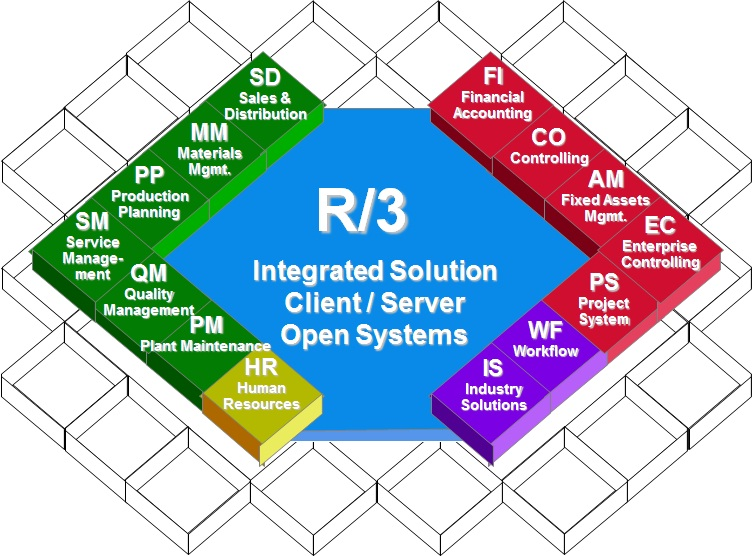
\includegraphics[width=1\textwidth]{images/sap_r3.jpg}
	\caption{Moduly SAP R3}
	\label{img:sapr3}
	\small
	fghfghgddh
\end{figure}

\section{SAP Plant Maintenance (PM)}
Modul SAP Plant Maintenance je komplexní řešení, které poskytuje nástroje pro kompletní údržbu v rámci firmy. Objekt údržby se skládá z technických objektů představujících strojní zařízení a skutečného modelu závodu.

Modul se skládá z činností jako je například správa technických objektů, zpracování údržby nebo preventivní údržba. Používá se k komplexnímu plánování, provádění denních činností údržby s integrací do ostatních SAP modulů.

\subsection{Technické objekty}
Pakliže je ve firmě zapotřebí správně nastavit DP (data processing) podporující údržbu, je nutné stávající technické systémy strukturovat na základě technických objektů. Vytvoření hierarchické podoby s sebou přináší následující výhody.
\begin{itemize}
	\item
	Doba potřebná pro správu technických objektů je snížena.
	\item
	Zpracování údržby je zjednodušeno.
	\item
	Doba strávená při zadávání dat během zpracování údržby je značně snížena.
	\item
	Konkrétnější, důkladnější a rychlejší vyhodnocení údajů o údržbě.
\end{itemize}

Technická správa objektů se skládá z následujících činností:
\begin{itemize}
	\item
	\textbf{Inspekce} - měřit a sledovat aktuální stav technického objektu
	\item
	\textbf{Preventivní údržba} - předvídat potřebu oprav a udržovat optimální stav technického objektu
	\item
	\textbf{Oprava} - měření a obnovení technického objektu
	\item
	\textbf{Další činnosti související s údržbou}
\end{itemize}
\vspace*{0.5cm}
Zpracování údržby pomáhá řídit skutečné údržbářské práce prováděné v údržbě. Proces se skládá ze tří oblastí:
\begin{itemize}
	\item
	\textbf{Upozornění na údržbu} -  oznamte poruchu nebo popište technickou podmínku objektu
	\item
	\textbf{Objednávka údržby} - provést podrobný plán údržby a sledovat průběh práce a uhradit náklady na údržbu
	\item
	\textbf{Historie údržby} - uložení důležitých údajů údržby pro vykazování a vyhodnocení
\end{itemize} 	

\subsection{Preventivní údržba}
Preventivní údržba je dlouhodobý proces, jehož cílem je zajistit vysokou použitelnost zařízení a funkčních míst a minimalizovat prostoje způsobené opravami. Tato funkce podporuje údržbu založenou na výkonu, pokud jsou měřicí body nebo čítače používány pro řízení technických podmínek objektu.
Součást preventivní údržby lze použít k:
\begin{itemize}
	\item
	Uložit seznam úkolů, které mají být provedeny
	\item
	Upřesněte rozsah inspekčních prací, preventivní údržbu a plánování činností
	\item
	Zadejte opakovanou frekvenci údržby
	\item
	Upřesněte přiřazení kontrolních činností a preventivní údržbu na základě nákladů
	\item
	Vyhodnotit náklady na budoucí preventivní údržbu a inspekční práci
\end{itemize} 	

Preventivní údržba v organizaci se používá k zabránění selhání systému a rozpadu výroby. Pomocí preventivní údržby můžete ve vaší organizaci dosáhnout různých výhod. Preventivní údržba se používá k provádění inspekcí, preventivní údržby a oprav. Plány údržby slouží k definování dat a rozsahu úkolů preventivní a inspekční údržby, které lze naplánovat pro technické objekty.

Seznam úkolů v Preventivní údržbě je definován jako sled činností, které jsou prováděny v rámci preventivní údržby v organizaci. Jsou používány k provádění opakovaných úkolů v rámci preventivní údržby a k jejich efektivnímu provedení.

Pomocí seznamů úkolů můžete snížit úsilí standardizací pracovní postup. Všechny aktualizace se provádějí na jednom konkrétním místě v seznamu úkolů údržby a všechny položky údržby a údržby v systému obdrží aktualizovaný stav pracovních postupů. Pomocí seznamů úkolů pomáhá při snižování úsilí potřebného pro vytvoření objednávek údržby a položek údržby, jak můžete vrátit do seznamu úkolů, abyste viděli pracovní postup.
Klíčové funkce seznamů úkolů v SAP Plant Maintenance jsou následující plánovaná a probíhající údržba podrobněji popsány v následujících odstavcích.

\paragraph{Plánovaná údržba}
Všechny plánované činnosti, jako je kontrola, údržba a opravy, jsou součástí plánované údržby. V údržbě rostlin definujete časové intervaly, kdy je třeba pracovní kroky provést a pracovní sekvence, ve kterých musí být provedeny. Seznamy úkolů jsou při plánování plánování údržby přiřazeny plánu údržby.

\paragraph{Probíhající údržba}
Seznam úkolů pro průběžnou údržbu obsahuje pracovní postupy založené na aktuální kontrole. Všechna kontrola, která se provádí bez pravidelného rozvrhu, je předmětem trvalé údržby.

\subsection{Zpracování údržby}
Zpracování údržby se skládá z několika úrovní, které nemusí být nutně plně realizovány.

Proto je možné zpracovat opravu v mnoha fázích plánování, jako je předběžná kalkulace, plánování práce, materiálové zabezpečení, plánování zdrojů a povolení. Je však také možné okamžitě reagovat na škody způsobené událostmi, které způsobí vypnutí výroby, a v co nejkratší možné době předložit požadované objednávky a prodejní doklady s minimálními údaji.

Zpracování údržby lze rozdělit na následující tři oblasti:
\begin{itemize}
	\item
	\textbf{Popis stavu objektu} - Nejdůležitějším prvkem v této oblasti je oznámení o údržbě. Používá se k popisu stavu technického objektu nebo hlášení poruchy na technickém objektu a požadavek na opravu poškození.
	\item
	\textbf{Provádění úkolů údržby} - Nejdůležitějším prvkem v této oblasti je objednávka údržby. Používá se k detailnímu plánování provádění údržbářských činností, sledování průběhu práce a vypořádání nákladů na údržbu.
	\item
	\textbf{Dokončení úkolů údržby} - Nejdůležitějším prvkem v této oblasti je historie údržby. Používá se k dlouhodobému uložení nejdůležitějších údajů o údržbě. Tyto údaje lze kdykoli vyžádat k vyhodnocení.
\end{itemize} 

Tyto prvky umožňují zpracovat všechny úkoly, které je třeba provést v údržbě zařízení, stejně jako operace, které nepatří přímo do údržby zařízení, jako jsou investice, restrukturalizace, úpravy a podobně.

\begin{figure}[H]
	\centering
	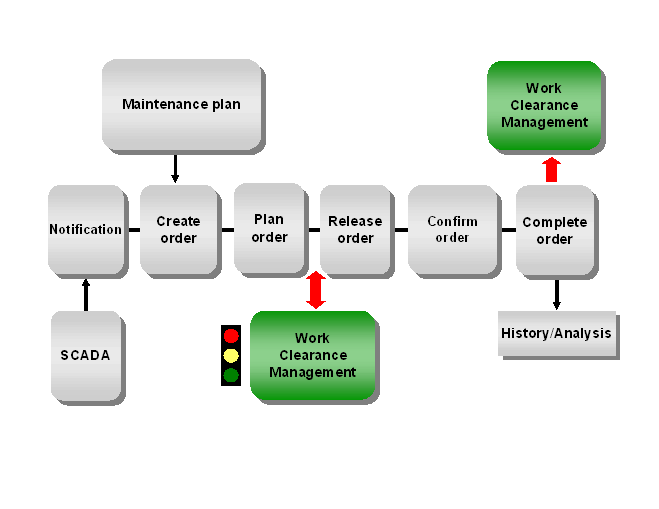
\includegraphics[width=1\textwidth]{images/pm_process.png}
	\caption{Moduly SAP R3}
	\label{img:sapr3}
	\small
	fghfghgddh
\end{figure}












\section{SAP BSP}

\section{SAP FIORI}

\chapter{Analýza a návrh aplikace}
Tato kapitola se věnuje analýze mnou navrženého řešení. Obsahuje jednotlivé podkapitoly zaměřující se na zpracování požadavků kladených na výslednou aplikaci, funkčnost RFID čtečky i návrh kompletního třídního modelu.	

\section{Model požadavků}
V této kapitole jsou uvedeny veškeré požadavky kladené na  výslednou aplikaci, které byly probírány se zadavatelem. Většina z nich byla stanovena ihned po určení rámcového zadání, některé však byly přidány nebo lehce upraveny v rámci konzultací , jak se upravovalo zadání práce. Následující výčet požadavků je rozdělen do dvou kategorií a to do funkčních a nefunkčních požadavků.  

\subsection{Funkční požadavky}
Funkční požadavky jsou rozděleny do 8 sekcí označených jako F1 až F8. 

\subsubsection{F1: Založení poruchy}
\subsubsection{F2: Založení požadavku na údržbu}
\subsubsection{F3: Zobrazení seznamu aktivních poruch}
\subsubsection{F4: Zobrazení seznamu historie poruch}
\subsubsection{F5: Zobrazení seznamu požadavků na údržbu}
\subsubsection{F6: Zobrazení seznamu prevencí}
\subsubsection{F7: Zobrazení dokumentace ke stroji (vybavení)}
\subsubsection{F8: Administrace uživatele}


\subsection{Nefunkční požadavky}

\subsubsection{N1: Grafické uživatelské rozhraní}
\subsubsection{N2: Provoz na provozních počítačích}
\subsubsection{N3: Provoz na mobilních zařízeních}
\subsubsection{N4: Dostupnost přes web}

\section{Model případů užití (Use Case model)}
Detailní specifikace funkčních požadavků, Typicky se jednotlivé požadavky rozpadají na několik případů užití. Základ pro tvorbu uživatelské příručky
– Podklady k tvorbě akceptačních testů
– Zpřesnění odhadů pracnosti
– Zadání pro programátora


\subsection{Seznam účastníků}

\begin{itemize}
	\item
	\textbf{Operátor výroby} - 
	\item
	\textbf{Údržbář} - 
	\item
	\textbf{Správce - Administrátor} - 
\end{itemize} 	

\subsection{Diagram případů užití}

\subsubsection{UC1: Vložit novou knihu}

\section{Návrh uživatelského rozhraní}

\subsection{Balsamiq}

\subsection{Built}

\subsection{Heuristická analýza}

\begin{enumerate}
	\item
	\textbf{Viditelnost stavu systému} -
	\item
	\textbf{Propojení systému a reálného světa} -
	\item
	\textbf{Uživatelská kontrola a svoboda} -
	\item
	\textbf{Standardizace a konzistence} -
	\item
	\textbf{Prevence chyb} -
	\item
	\textbf{Rozpoznání namísto vzpomínání} -
	\item
	\textbf{Flexibilní a efektivní použití} -
	\item
	\textbf{Estetický a minimalistický} -
	\item
	\textbf{Pomoc uživatelů pochopit, poznat a vzpamatovat se z chyb} -
	\item
	\textbf{Nápověda a návody} -
\end{enumerate} 

\chapter{Návrh architektury}

\chapter{Implementace}

\section{Porovnání vývojových prostředí}

\section{Doporučení pro vývoj}

\begin{conclusion}
	%sem napište závěr Vaší práce
\end{conclusion}

\bibliographystyle{csn690}
\bibliography{mybibliographyfile}

\appendix

\chapter{Seznam použitých zkratek}
% \printglossaries
\begin{description}
	\item[GUI] Graphical user interface
	\item[XML] Extensible markup language
\end{description}


% % % % % % % % % % % % % % % % % % % % % % % % % % % % 
% % Tuto kapitolu z výsledné práce ODSTRAŇTE.
% % % % % % % % % % % % % % % % % % % % % % % % % % % % 
% 
% \chapter{Návod k~použití této šablony}
% 
% Tento dokument slouží jako základ pro napsání závěrečné práce na Fakultě informačních technologií ČVUT v~Praze.
% 
% \section{Výběr základu}
% 
% Vyberte si šablonu podle druhu práce (bakalářská, diplomová), jazyka (čeština, angličtina) a kódování (ASCII, \mbox{UTF-8}, \mbox{ISO-8859-2} neboli latin2 a nebo \mbox{Windows-1250}). 
% 
% V~české variantě naleznete šablony v~souborech pojmenovaných ve formátu práce\_kódování.tex. Typ může být:
% \begin{description}
% 	\item[BP] bakalářská práce,
% 	\item[DP] diplomová (magisterská) práce.
% \end{description}
% Kódování, ve kterém chcete psát, může být:
% \begin{description}
% 	\item[UTF-8] kódování Unicode,
% 	\item[ISO-8859-2] latin2,
% 	\item[Windows-1250] znaková sada 1250 Windows.
% \end{description}
% V~případě nejistoty ohledně kódování doporučujeme následující postup:
% \begin{enumerate}
% 	\item Otevřete šablony pro kódování UTF-8 v~editoru prostého textu, který chcete pro psaní práce použít -- pokud můžete texty s~diakritikou normálně přečíst, použijte tuto šablonu.
% 	\item V~opačném případě postupujte dále podle toho, jaký operační systém používáte:
% 	\begin{itemize}
% 		\item v~případě Windows použijte šablonu pro kódování \mbox{Windows-1250},
% 		\item jinak zkuste použít šablonu pro kódování \mbox{ISO-8859-2}.
% 	\end{itemize}
% \end{enumerate}
% 
% 
% V~anglické variantě jsou šablony pojmenované podle typu práce, možnosti jsou:
% \begin{description}
% 	\item[bachelors] bakalářská práce,
% 	\item[masters] diplomová (magisterská) práce.
% \end{description}
% 
% \section{Použití šablony}
% 
% Šablona je určena pro zpracování systémem \LaTeXe{}. Text je možné psát v~textovém editoru jako prostý text, lze však také využít specializovaný editor pro \LaTeX{}, např. Kile.
% 
% Pro získání tisknutelného výstupu z~takto vytvořeného souboru použijte příkaz \verb|pdflatex|, kterému předáte cestu k~souboru jako parametr. Vhodný editor pro \LaTeX{} toto udělá za Vás. \verb|pdfcslatex| ani \verb|cslatex| \emph{nebudou} s~těmito šablonami fungovat.
% 
% Více informací o~použití systému \LaTeX{} najdete např. v~\cite{wikilatex}.
% 
% \subsection{Typografie}
% 
% Při psaní dodržujte typografické konvence zvoleného jazyka. České \uv{uvozovky} zapisujte použitím příkazu \verb|\uv|, kterému v~parametru předáte text, jenž má být v~uvozovkách. Anglické otevírací uvozovky se v~\LaTeX{}u zadávají jako dva zpětné apostrofy, uzavírací uvozovky jako dva apostrofy. Často chybně uváděný symbol "{} (palce) nemá s~uvozovkami nic společného.
% 
% Dále je třeba zabránit zalomení řádky mezi některými slovy, v~češtině např. za jednopísmennými předložkami a spojkami (vyjma \uv{a}). To docílíte vložením pružné nezalomitelné mezery -- znakem \texttt{\textasciitilde}. V~tomto případě to není třeba dělat ručně, lze použít program \verb|vlna|.
% 
% Více o~typografii viz \cite{kobltypo}.
% 
% \subsection{Obrázky}
% 
% Pro umožnění vkládání obrázků je vhodné použít balíček \verb|graphicx|, samotné vložení se provede příkazem \verb|\includegraphics|. Takto je možné vkládat obrázky ve formátu PDF, PNG a JPEG jestliže používáte pdf\LaTeX{} nebo ve formátu EPS jestliže používáte \LaTeX{}. Doporučujeme preferovat vektorové obrázky před rastrovými (vyjma fotografií).
% 
% \subsubsection{Získání vhodného formátu}
% 
% Pro získání vektorových formátů PDF nebo EPS z~jiných lze použít některý z~vektorových grafických editorů. Pro převod rastrového obrázku na vektorový lze použít rasterizaci, kterou mnohé editory zvládají (např. Inkscape). Pro konverze lze použít též nástroje pro dávkové zpracování běžně dodávané s~\LaTeX{}em, např. \verb|epstopdf|.
% 
% \subsubsection{Plovoucí prostředí}
% 
% Příkazem \verb|\includegraphics| lze obrázky vkládat přímo, doporučujeme však použít plovoucí prostředí, konkrétně \verb|figure|. Například obrázek \ref{fig:float} byl vložen tímto způsobem. Vůbec přitom nevadí, když je obrázek umístěn jinde, než bylo původně zamýšleno -- je tomu tak hlavně kvůli dodržení typografických konvencí. Namísto vynucování konkrétní pozice obrázku doporučujeme používat odkazování z~textu (dvojice příkazů \verb|\label| a \verb|\ref|).
% 
% \begin{figure}\centering
% 	
\includegraphics[width=0.5\textwidth, angle=30]{cvut-logo-bw}
% 	\caption[Příklad obrázku]{Ukázkový obrázek v~plovoucím prostředí}\label{fig:float}
% \end{figure}
% 
% \subsubsection{Verze obrázků}
% 
% % Gnuplot BW i barevně
% Může se hodit mít více verzí stejného obrázku, např. pro barevný či černobílý tisk a nebo pro prezentaci. S~pomocí některých nástrojů na generování grafiky je to snadné.
% 
% Máte-li například graf vytvořený v programu Gnuplot, můžete jeho černobílou variantu (viz obr. \ref{fig:gnuplot-bw}) vytvořit parametrem \verb|monochrome dashed| příkazu \verb|set term|. Barevnou variantu (viz obr. \ref{fig:gnuplot-col}) vhodnou na prezentace lze vytvořit parametrem \verb|colour solid|.
% 
% \begin{figure}\centering
% 	\includegraphics{gnuplot-bw}
% 	\caption{Černobílá varianta obrázku generovaného programem Gnuplot}\label{fig:gnuplot-bw}
% \end{figure}
% 
% \begin{figure}\centering
% 	\includegraphics{gnuplot-col}
% 	\caption{Barevná varianta obrázku generovaného programem Gnuplot}\label{fig:gnuplot-col}
% \end{figure}
% 
% 
% \subsection{Tabulky}
% 
% Tabulky lze zadávat různě, např. v~prostředí \verb|tabular|, avšak pro jejich vkládání platí to samé, co pro obrázky -- použijte plovoucí prostředí, v~tomto případě \verb|table|. Například tabulka \ref{tab:matematika} byla vložena tímto způsobem.
% 
% \begin{table}\centering
% 	\caption[Příklad tabulky]{Zadávání matematiky}\label{tab:matematika}
% 	\begin{tabular}{|l|l|c|c|}\hline
% 		Typ		& Prostředí		& \LaTeX{}ovská zkratka	& \TeX{}ovská zkratka	\tabularnewline \hline \hline
% 		Text		& \verb|math|		& \verb|\(...\)|	& \verb|$...$|		\tabularnewline \hline
% 		Displayed	& \verb|displaymath|	& \verb|\[...\]|	& \verb|$$...$$|	\tabularnewline \hline
% 	\end{tabular}
% \end{table}
% 
% % % % % % % % % % % % % % % % % % % % % % % % % % % % 

\chapter{Obsah přiloženého CD}

%upravte podle skutecnosti

\begin{figure}
	\dirtree{%
		.1 readme.txt\DTcomment{stručný popis obsahu CD}.
		.1 exe\DTcomment{adresář se spustitelnou formou implementace}.
		.1 src.
		.2 impl\DTcomment{zdrojové kódy implementace}.
		.2 thesis\DTcomment{zdrojová forma práce ve formátu \LaTeX{}}.
		.1 text\DTcomment{text práce}.
		.2 thesis.pdf\DTcomment{text práce ve formátu PDF}.
		.2 thesis.ps\DTcomment{text práce ve formátu PS}.
	}
\end{figure}

\end{document}
